\documentclass[12pt,letterpaper]{article}
\usepackage{fullpage}
\usepackage[top=2cm, bottom=4.5cm, left=2.5cm, right=2.5cm]{geometry}
\usepackage{amsmath,amsthm,amsfonts,amssymb,amscd}
\usepackage{lastpage}
\usepackage{enumerate}
\usepackage{fancyhdr}
\usepackage{mathrsfs}
\usepackage{graphicx}
%% download this package and put it in the same directory as this file
\setlength{\parindent}{0.0in}
\setlength{\parskip}{0.05in}

\usepackage{subfigure}
\usepackage{float}
\usepackage{multicol}
\usepackage{multirow}
\usepackage{enumitem}
% Edit these as appropriate
\newcommand\course{DATA1050}
\newcommand\semester{Fall 2019}
\newcommand\hwnumber{3}
\newcommand\Name{Tongxin Wang}           % <-- Fill in your name here

\pagestyle{fancyplain}
\headheight 35pt
\lhead{\Name}
\chead{\textbf{\Large Project \hwnumber}}
\rhead{\course\;--\;\semester \\ \today}
\lfoot{}
\cfoot{}
\rfoot{\small\thepage}
\headsep 1.5em

\begin{document}

% Start editing here! Each section corresponds to a question.
\section{Time Complexity}
This is a \textbf{DATA1050} \LaTeX template to show you some syntax in LaTeX.

You can write your answer in plain text.

\begin{enumerate}
    \item For Merge sort, the average runtime complexity is $O(NlogN)$, the worst case runtime complexity is $O(NlogN)$
    
    \item For quick sort, the averge runtime complexity is $O(NlogN)$, the worst case runtime complexity is $O(N^2)$
    
    \item For insertion sort, both the average runtime complexity and the worst case runtime complexity are $O(N^2)$
    \item The Merge sort and the Quick sort would require extra spaces as their space complexities are $O(N)$
    
\end{enumerate}

\pagebreak
\section{Recursive Calls}
$merge\_sort(A, 0, 128) \rightarrow merge\_sort(A, 0, 64) \rightarrow merge\_sort(A, 0, 32) \rightarrow merge\_sort(A, 32, 64) \rightarrow merge\_sort(A, 64, 128) \rightarrow merge\_sort(A, 64, 96) \rightarrow merge\_sort(A, 96, 128)$
\pagebreak
\section{Base Cases}
The base case of the orignal sort is when the lengths of all sublists are 1; the base case of hybrid sort is when the length of the sublist is no greater than threshold.
\pagebreak
\section{Unittests}
For insertion sort inplace, I tested with lists of length 0 and 1, and I testes with identical lists (where all the elements are the same) and normal lists.\newline
For merge inplace, I tested with lists of length 0 and 1, and I testes with identical lists (where all the elements are the same) and normal lists.\newline
For hybrid sort, I tested with lists of length 0 and 1, and I testes with identical lists (where all the elements are the same) and normal lists.\newline
 
\pagebreak
\section{Parameter Tuning}
The best parameter I found is 16. \newline
\begin{figure}[H]
    \centering
    % replace "dim.png" with your image file, placed in the same directory
    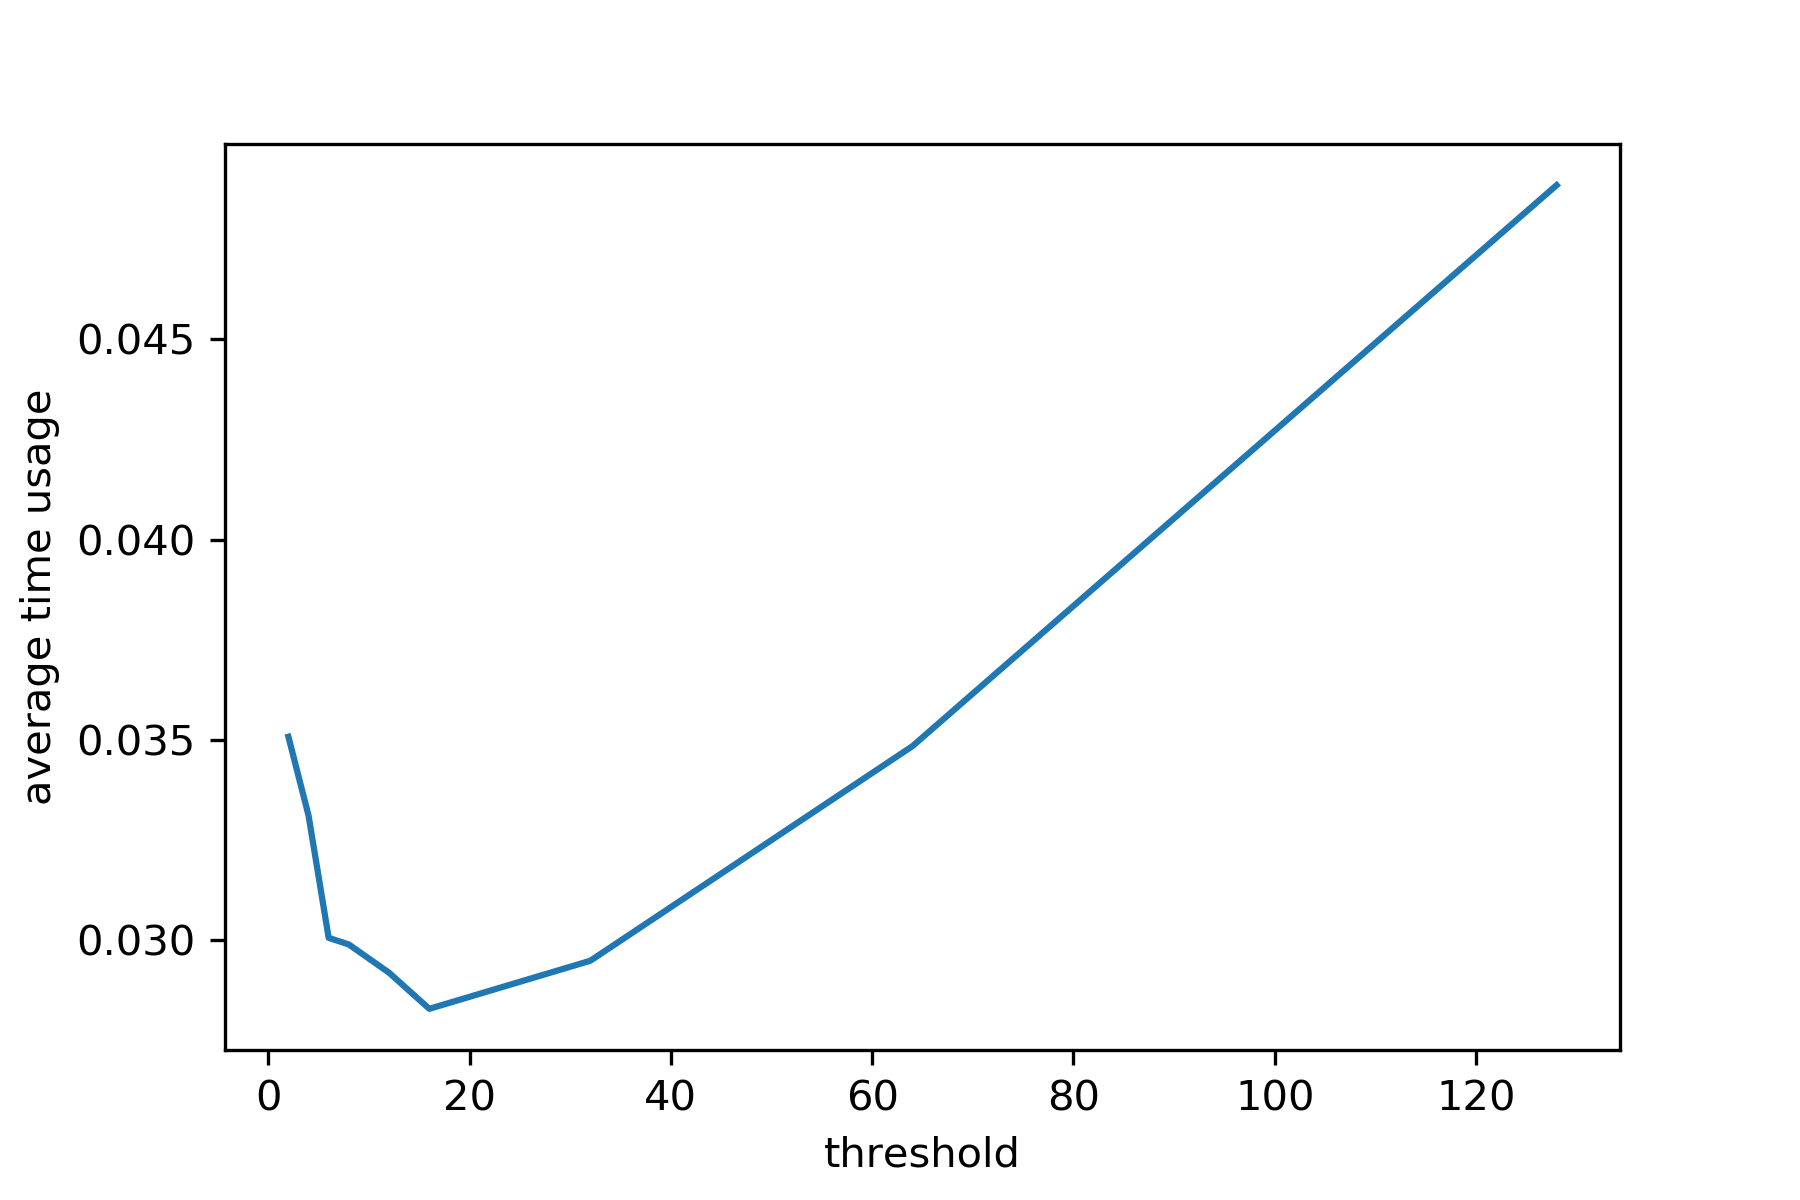
\includegraphics[width=0.6\linewidth]{dim.png}
    % give it a name
    \caption{My Plot for hw3}
\end{figure}

\pagebreak
\section{Too Big To Sort}
a. First we create a temporpary list to store the sorted elements from the k listes. For k sorted lists, we compare the first index of each list, and append the smallest into the temporary list, and we update the corresponding index. After finish comparision, if we still have lists which have elements that did not append to the temporpary list, we append the rest of the list to the temporary list. In the end, the temporary array is a sorted list. Let's say the total length of k lists is n. The time acmplexity is $O(kn)$, and the space complexity is $O(n)$ \newline
b. First we sort each small files, and they are stored in the hard disk. We create a csv file to store the sorted numbers instead of a list, and the file is stored on the hard drive. When we merge all the files using the method we described in $(a)$, since only a few index of elements being compared are stores in the RAM (other infomation is stored on disk), the space we are using is only a small part of the RAM.\newline
c. First we create 100 buckets and the buckets $(csv files)$ to hold numbers in the interval $[0,1], (1,2], \dots, (99,100]$, then get the integer part of each number using method int(num) , and we put the numbers into their corresponding files by comparing them to the intervals. The intervals are stored on the RAM, but they only take small spaces of the RAM. These 100 files are stored on the hard disk. Then we sort each files, where each file is less than 2GB, and we will get 100 sorted files and they form a sorted array when concatenated.\newline
\end{document}